% ============================================================
%  附录D 相互作用电子系统中的谱函数（原书印刷页 547–551）
%  底本：高等教育出版社《固体理论》第二版
%  （PDF 页 = 印刷页 + 20，原书 PDF 页 567–571；
%  任务单所记"附录D PDF 567–569"缺 p570–571 两页，
%  (D.17) 第二行起至 (D.24) 实在 p570–571，已照原书补齐）
%  公式编号自检：全附录 (D.1)–(D.24) 连续 24 个，无缺号，
%    与任务单 tags=24 一致。
%
%  已修正的 OCR/原书错误（除全角句点转"."、删 ~ 间隔符、
%  拆开行内公式与中文等常规项外）：
%  1. (D.1) 矩阵元 OCR"C_{kα}"按 p567 复原为 C_{kσ}；
%     (D.17) 跨页两行（p569 页末 + p570 页首）已并为一式。
%  2. p567 段中"并 n_{kσ} 取 h=1 单位后"OCR 语序错乱，按原书
%     复原为"并取 ħ=1 单位后可由式(A.28)求得"。
%  3. (D.5) OCR"A^-(k,ω)、f^-(ω/ω)"乱码按 p568 复原为
%     A(k,ω)、f(ω)。
%  4. 原书 p568 (D.6) 右端印 Im G_r(ω) 漏宗量 k（左端求和号下
%     已显含 k），按上下文补为 Im G_r(k,ω)。
%  5. 原书 p568 (D.7) 积分内 A(ω') 漏宗量 k，按 (D.9)(D.11)
%     同类积分补为 A(k,ω')。
%  6. 原书 p568 (D.9) 中间项 G_a(ω) 漏宗量 k，按左端补为
%     G_a(k,ω)。
%  7. 原书 p569 (D.16) 之下行文印"G_r^{(0)}(r,ω)在上半面又无
%     极点"，r 为 k 之误（本节通篇讨论动量 k 电子），改 (k,ω)。
%  8. p570 段中"其寿命正比于Γ-1．在格林函数理 Γ_k^{-1} 论中"
%     OCR 把 Γ_k^{-1} 错位到下句，按 p570 归还为"其寿命正比于
%     Γ_k^{-1}．在格林函数理论中"。
%  9. (D.20) OCR"T_k"为 Γ_k 之误识，全节统一 Γ_k；
%     (D.15)(D.18)(D.23) OCR"(σ−1/π)""(ω−1/π)"等按原书复原为
%     (−1/π)。
% 10. (D.24) 自能虚部取点原书作 ω=Ẽ_k（OCR 亦含波浪号），与
%     (D.20) 之 ω=E_k 并存，系原书照排，均照录未改。
% 11. 体例：< <A|B> > 统一 \langle\langle…\rangle\rangle；虚单位
%     i、指数底 e 用正体；宗量 k 用粗体（照原书）。
%  插图：图 D.1 电子的谱函数（原书印刷 p550/PDF p570），
%  占位图 figures/figD-1.pdf，待重绘代理按原书绘制。
%  遗留问题：
%  · (D.20)(D.24) 自能虚部取点一处作 ω=E_k、一处作 ω=Ẽ_k，
%    原书如此，照录未改。
% ============================================================
\chapter{相互作用电子系统中的谱函数}

由于固体量子论的许多问题均涉及附录 A 中所引进的谱函数，特别是相互作用电子系统的谱函数，因此有必要对它的某些重要的基本属性作专门介绍. 根据式(A.30)，令算符 $A=C_{k\sigma}$ 与 $B=C_{k\sigma}^{+}$ 并取 $\hbar=1$ 单位，可将电子系统的谱函数定义为
\begin{equation}
A(\boldsymbol{k},\omega)\equiv Z_{\mathrm{G}}^{-1}
\sum_{n,m}\mathrm{e}^{-\beta E_{n}'}
|\langle n|C_{k\sigma}^{+}|m\rangle|^{2}
\bigl(\mathrm{e}^{\beta(\omega-\mu)}+1\bigr)
\delta(\omega-E_{n}+E_{m})
\end{equation}
其中取 $+$ 号是因为费密子系统满足反对易关系
$[C_{k\sigma},C_{k\sigma}^{+}]_{+}=1$. 由于在定义式(D.1)右边求和号内所有的因子均为正，可以断言 $A(\boldsymbol{k},\omega)$ 对于变量 $\boldsymbol{k}$ 及 $\omega$ 的所有取值都是正的. 按此，电子系统的谱函数具有下列正定性：
\begin{equation}
A(\boldsymbol{k},\omega)\geqslant 0
\end{equation}
由于正定性，$A(\boldsymbol{k},\omega)$ 又可称为谱权重函数或谱密度函数，相应于式(A.31)的电子系统的谱函数求和律可写成下列具体表示式：
\begin{equation}
\int_{-\infty}^{\infty}\mathrm{d}\omega\,A(\boldsymbol{k},\omega)
=\langle[C_{k\sigma},C_{k\sigma}^{+}]_{+}\rangle=1
\end{equation}
它可以理解为谱密度函数的归一性条件. 再利用谱定理讨论
$(\boldsymbol{k},\sigma)$ 态上的平均电子数 $n_{k\sigma}$ 的表示式，这时若将式(A.19)推广到巨正则系综，并取 $\hbar=1$ 单位后可由式(A.28)求得
\begin{equation}
n_{k\sigma}=\langle C_{k\sigma}^{+}C_{k\sigma}\rangle
=\int_{-\infty}^{\infty}\mathrm{d}\omega\,
\frac{A(\boldsymbol{k},\omega)}{\mathrm{e}^{\beta(\omega-\mu)}+1}
=\int_{-\infty}^{\infty}\mathrm{d}\omega\,
f(\omega)A(\boldsymbol{k},\omega)
\end{equation}
其中 $f(\omega)$ 为费密分布函数. 根据上式的最后一个等式，谱函数的确切物理意义可解释为给定自旋的电子在状态空间 $\boldsymbol{k}$ 点的态密度. 目前在研究强关联电子系统时，已发展了角分辨光发射谱技术，可用作直接测量互作用电子系统的谱函数.

利用谱函数还可以直接导出互作用电子系统的态密度. 对于含 $N$ 个格点的晶格系统，利用平移对称性和式(D.4)可确定每个格点上 $\sigma$ 自旋电子的平均数
\begin{equation}
\begin{aligned}
n_{\sigma}&=N^{-1}\sum_{j}\langle C_{j\sigma}^{+}C_{j\sigma}\rangle
=N^{-1}\sum_{k}\langle C_{k\sigma}^{+}C_{k\sigma}\rangle\\
&=\int_{-\infty}^{\infty}\mathrm{d}\omega\,f(\omega)
\biggl\{N^{-1}\sum_{k}A(\boldsymbol{k},\omega)\biggr\}\\
&=\int_{-\infty}^{\infty}\mathrm{d}\omega\,f(\omega)\rho_{\sigma}(\omega)
\end{aligned}
\end{equation}
其中 $\rho_{\sigma}(\omega)$ 恰好代表平均每个格点上 $\sigma$ 自旋电子在单位能量间隔内的状态数，此即第十一章§1中所定义的局域态密度（LDOS）. 显然，局域态密度可以用 $A(\boldsymbol{k},\omega)$ 表示
\begin{equation}
\rho_{\sigma}(\omega)=\frac{1}{N}\sum_{k}A(\boldsymbol{k},\omega)
=-\biggl(\frac{1}{\pi N}\biggr)\sum_{k}
\mathrm{Im}G_{\mathrm{r}}(\boldsymbol{k},\omega)
\end{equation}
这是固体理论中的一个十分有用的公式.

谱函数的引入对于讨论单电子格林函数的基本属性和相互作用电子系统中准电子的特征都是十分方便的，现分别介绍如下：

\subsection*{1. 基本属性}

根据附录 A 中的式(A.26)、(A.27)和(A.30)，可求得推迟与超前格林函数的莱曼积分表示式
\begin{equation}
G_{\mathrm{r}(a)}(\boldsymbol{k},\omega)
\equiv\langle\langle C_{k\sigma}|C_{k\sigma}^{+}\rangle\rangle_{\omega\pm\mathrm{i}\eta}
=\int_{-\infty}^{\infty}\mathrm{d}\omega'\,
\frac{A(\boldsymbol{k},\omega')}{\omega-\omega'\pm\mathrm{i}\eta}
\end{equation}
这是一个十分简明的公式. 由式(D.7)立刻求得，当 $\omega$ 取实数时推迟和超前格林函数的实部相等，但虚部异号，表明 $G_{\mathrm{r}}$ 与 $G_{\mathrm{a}}$ 分别位于实轴的两侧
\begin{equation}
\left.
\begin{aligned}
&\mathrm{Re}G_{\mathrm{r}}(\boldsymbol{k},\omega)
=\mathrm{Re}G_{\mathrm{a}}(\boldsymbol{k},\omega)\\
&\mathrm{Im}G_{\mathrm{r}}(\boldsymbol{k},\omega)
=-\pi A(\boldsymbol{k},\omega)\\
&\mathrm{Im}G_{\mathrm{a}}(\boldsymbol{k},\omega)
=+\pi A(\boldsymbol{k},\omega)
\end{aligned}
\right\}
\end{equation}
这正是实轴应取为割线的根本原因. 从莱曼表示的积分公式(D.7)和谱函数的求和律式(D.3)又可以进一步确定双时格林函数在无穷远点（$|\omega|\to\infty$ 时）的渐近行为
\begin{equation}
\lim_{|\omega|\to\infty}G_{\mathrm{r}}(\boldsymbol{k},\omega)
=\lim_{|\omega|\to\infty}G_{\mathrm{a}}(\boldsymbol{k},\omega)
\sim\frac{1}{\omega}\int_{-\infty}^{\infty}
\mathrm{d}\omega'\,A(\boldsymbol{k},\omega')\sim\frac{1}{\omega}
\end{equation}
表明格林函数在无限远点的重要收敛特性已包括在用 $A(\boldsymbol{k},\omega)$ 描述的莱曼积分公式(D.7)之中了. 此外，利用莱曼积分表示式还可以导出著名的色散关系. 从式(D.7)出发利用数学公式
\begin{equation}
\lim_{\eta\to 0}\frac{1}{x+\mathrm{i}\eta}
=\mathcal{P}\biggl(\frac{1}{x}\biggr)-\mathrm{i}\pi\delta(x)
\end{equation}
得到
\begin{equation}
G_{\mathrm{r}}(\boldsymbol{k},\omega)=\mathcal{P}
\int_{-\infty}^{\infty}\mathrm{d}\omega'\,
\frac{A(\boldsymbol{k},\omega')}{\omega-\omega'}
-\mathrm{i}\pi A(\boldsymbol{k},\omega)
\end{equation}
再考虑到电子的 $A(\boldsymbol{k},\omega)$ 为正实量，并利用式(D.8)又可求得一个重要的关系式
\begin{equation}
\begin{aligned}
\mathrm{Re}G_{\mathrm{r}}(\boldsymbol{k},\omega)
&=\mathcal{P}\int_{-\infty}^{\infty}\mathrm{d}\omega'\,
\frac{A(\boldsymbol{k},\omega')}{\omega-\omega'}\\
&=\frac{1}{\pi}\int_{-\infty}^{\infty}\mathrm{d}\omega'\,
\mathrm{Im}G_{\mathrm{r}}(\boldsymbol{k},\omega')
\mathcal{P}\biggl(\frac{1}{\omega'-\omega}\biggr)
\end{aligned}
\end{equation}
这就是双时推迟格林函数的色散关系. 在历史上，克喇末和克朗尼格（Kronig）首先证明：对于任意的上半复平面解析函数 $B(\omega)$，当 $|\omega|\to\infty$ 具有收敛性 $B(\omega)\to 0$ 时，存在类似的色散关系
\begin{equation}
\mathrm{Re}B(\omega)=\frac{1}{\pi}\int_{-\infty}^{\infty}
\mathrm{d}\omega'\,\mathrm{Im}B(\omega')
\mathcal{P}\biggl(\frac{1}{\omega'-\omega}\biggr)
\end{equation}
因此，人们又将色散关系称为克喇末-克朗尼格关系.

\subsection*{2. 准电子特征}

对于无相互作用的自由电子系统，附录 C 中已从运动方程求出了其格林函数
\begin{equation}
G_{\mathrm{r}}^{(0)}(\boldsymbol{k},\omega)
=\frac{1}{\omega-E_{k}+\mathrm{i}\eta}
\end{equation}
其中 $E_{k}=k^{2}/2m$，$\eta=+0$. 由此又可得自由电子的谱函数
\begin{equation}
A^{(0)}(\boldsymbol{k},\omega)=\bigl(-1/\pi\bigr)
\mathrm{Im}G_{\mathrm{r}}^{(0)}(\boldsymbol{k},\omega)
=\delta(\omega-E_{k})
\end{equation}
是一个 $\delta$ 函数. 在 $A$-$\omega$ 平面上自由电子的谱函数是一个宽度为零的尖峰，峰的中心位于 $\omega=E_{k}$ 处，表明一个具有确定 $\boldsymbol{k}$ 值的自由电子只对应于一个确定的能量值 $\omega=E_{k}$ 和无限长寿命的稳定电子态，这一点还可以从 $G_{\mathrm{r}}^{(0)}(\boldsymbol{k},\omega)$ 的傅里叶变换看出
\begin{equation}
\begin{aligned}
G_{\mathrm{r}}^{(0)}(\boldsymbol{k},t)&=\frac{1}{2\pi}
\int_{-\infty}^{\infty}\mathrm{d}\omega\,
G_{\mathrm{r}}^{(0)}(\boldsymbol{k},\omega)\mathrm{e}^{-\mathrm{i}\omega t}\\
&=-\mathrm{i}\theta(t)\mathrm{e}^{-\mathrm{i}E_{k}t}
\end{aligned}
\end{equation}
其中 $\theta(t)$ 因子的出现是由于 $G_{\mathrm{r}}^{(0)}(\boldsymbol{k},\omega)$ 的极点在下半面 $\omega=E_{k}-\mathrm{i}\eta$ 处，当 $t>0$ 时应绕下半复平面作回路积分求出 $(-\mathrm{i}\mathrm{e}^{-\mathrm{i}E_{k}t})$ 留数，而 $t<0$ 只能绕上半复平面作回路积分，而 $G_{\mathrm{r}}^{(0)}(\boldsymbol{k},\omega)$ 在上半面又无极点，因此 $t<0$ 时积分为零. 式(D.16)清楚地表明动量为 $\boldsymbol{k}$ 的自由电子以 $\omega=E_{k}$ 能量传播而无阻尼.

对于相互作用的电子系统，根据戴逊方程式(C.21)
\begin{equation}
\begin{aligned}
G_{\mathrm{r}}(\boldsymbol{k},\omega)
&=[\omega-E_{k}-\Sigma_{\mathrm{r}}(\boldsymbol{k},\omega)]^{-1}\\
&=[\omega-E_{k}-\mathrm{Re}\Sigma_{\mathrm{r}}(\boldsymbol{k},\omega)
-\mathrm{i}\,\mathrm{Im}\Sigma_{\mathrm{r}}(\boldsymbol{k},\omega)]^{-1}
\end{aligned}
\end{equation}
其谱函数
\begin{equation}
A(\boldsymbol{k},\omega)=
\frac{(-1/\pi)\,\mathrm{Im}\Sigma_{\mathrm{r}}(\boldsymbol{k},\omega)}
{\left[\omega-E_{k}-\mathrm{Re}\Sigma_{\mathrm{r}}(\boldsymbol{k},\omega)\right]^{2}
+\left[\mathrm{Im}\Sigma_{\mathrm{r}}(\boldsymbol{k},\omega)\right]^{2}}
\end{equation}
从正定性 $A(\boldsymbol{k},\omega)>0$ 可知，双时推迟格林函数的自能虚部应为负，即 $\mathrm{Im}\Sigma_{\mathrm{r}}(\boldsymbol{k},\omega)<0$，相应的在 $G_{\mathrm{r}}(\boldsymbol{k},\omega)$ 的分母中仅会出现正的虚数项. 自能的实部 $\mathrm{Re}\Sigma_{\mathrm{r}}(\boldsymbol{k},\omega)$ 将对未微扰电子的能量 $E_{k}$ 产生修正，使 $E_{k}$ 变为
\begin{equation}
\widetilde{E}_{k}=E_{k}+\mathrm{Re}\Sigma_{\mathrm{r}}(\boldsymbol{k},\omega)
\end{equation}
而自能虚部的贡献在式(D.17)中可归结为 $+\mathrm{i}\Gamma_{k}$，其中
\begin{equation}
\Gamma_{k}\equiv-\mathrm{Im}\Sigma_{\mathrm{r}}
(\boldsymbol{k},\omega=E_{k})
\end{equation}
按此，互作用系统中的单电子格林函数可以近似写成下列简单表示式
\begin{equation}
G_{\mathrm{r}}(\boldsymbol{k},\omega)
\approx 1/(\omega-\widetilde{E}_{k}+\mathrm{i}\Gamma_{k})
\end{equation}
它描述互作用系统中的准粒子行为. 对上式作傅里叶变换求出含时间的 $\boldsymbol{k}$ 电子格林函数
\begin{equation}
G_{\mathrm{r}}(\boldsymbol{k},t)\approx\frac{1}{2\pi}
\int_{-\infty}^{\infty}\mathrm{d}\omega\,
\frac{\mathrm{e}^{-\mathrm{i}\omega t}}
{\omega-\widetilde{E}_{k}+\mathrm{i}\Gamma_{k}}
=-\mathrm{i}\theta(t)\mathrm{e}^{-\mathrm{i}\widetilde{E}_{k}t}
\mathrm{e}^{-\Gamma_{k}t}
\end{equation}
显然，$\boldsymbol{k}$ 电子在传播过程中将衰减，其寿命正比于
$\Gamma_{k}^{-1}$. 在格林函数理论中，通常将谱函数 $A(\boldsymbol{k},\omega)$ 的峰宽之倒数定义为准粒子的寿命. 在这里电子谱函数可从式(D.21)求出为
\begin{equation}
\begin{aligned}
A(\boldsymbol{k},\omega)&=-\frac{1}{\pi}
\mathrm{Im}G_{\mathrm{r}}(\boldsymbol{k},\omega)\\
&=\frac{\left(\Gamma_{k}/\pi\right)}
{\left(\omega-\widetilde{E}_{k}\right)^{2}+\Gamma_{k}^{2}}
\end{aligned}
\end{equation}
如图 D.1 所示，是一个峰宽为 $2\Gamma_{k}$ 的共振峰. 因此准粒子的寿命 $\tau_{k}=1/(2\Gamma_{k})$，从而得到自能虚部与 $\tau_{k}$ 的关系

\begin{center}
\begin{minipage}{7.5cm}
\centering
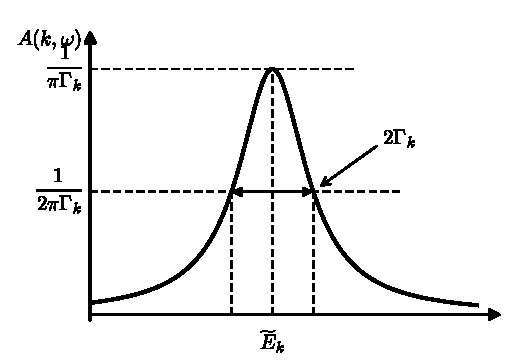
\includegraphics[width=7.5cm]{figD-1.pdf}\\{\small 图 D.1\quad 电子的谱函数}
\end{minipage}
\end{center}

\begin{equation}
1/\tau_{k}=2\Gamma_{k}\equiv-2\,\mathrm{Im}\Sigma_{\mathrm{r}}
(\boldsymbol{k},\omega=\widetilde{E}_{k})
\end{equation}
这是一个重要的关系式，在第四章§11中，我们将利用无规相近似介电函数计算寿命，然后由上式决定
$\mathrm{Im}\Sigma_{\mathrm{r}}(\boldsymbol{k},\widetilde{E}_{k})$.
